\documentclass[12pt]{article}
\usepackage[utf8]{inputenc}
\usepackage{graphicx}
\usepackage[hidelinks]{hyperref}
\usepackage{geometry}
\usepackage{url}
\geometry{a4paper, margin=1in}

\title{Java 2D\&3D Graphics Project1}
\author{m5271506 Kiyohiro Murai}
\date{2023-12-27}

\begin{document}

\maketitle
\tableofcontents
\newpage

\section{Classes}
Please see code for details. Here it will be written an overview of each class.
\subsection{ContourPlotMain.java}
Class containing the main method. Controls GUI construction, data reading, etc. It is responsible for arranging the contour panels described later in the JFrame and visually displaying it.
\subsection{ContourLinePlotPanel.java}
Panel to draw contour lines. Create a panel that draws contour lines based on the shape data read from the vtk file, the color data from the color map csv file and isoValues.
\subsection{FilledContourPlotPanel.java}
Create a panel to draw filled contour lines. The data also used is vtk and color map csv.
\subsection{Point.java}
A class that handles the point of shapes. This class has x, y, z=0 and scalar values defined as fields. Additionally, it includes methods to normalize a scalar value to correspond to an isoValues and to scale it to fit the JPanel size.
\subsection{Triangle.java}
A triangle class with three Point.java instances.
\subsection{ColorMap.java}
This is a class for handling colors with specific scalar values from the provided color map csv. Since scalar values are specified in the range [0-1] in csv, it includes a method to normalize to correspond to the scalar values of the shape data.
\subsection{VTKReader.java}
This is a class that reads vtk files and obtains graphic data as Java objects. Get all points, triangles, cell types, max-min points to normalize, max-min scalar values to normalize.
\subsection{ColorMapReader.java}
This is a class for reading colormap csv and handling colors with specific scalar values using Java objects.

\section{Contour plotting algorithm}
ContourLinePlotPanel.java has a drawContourLines() method to draw contour lines. Draws contour lines from the triangles, colormap, and isoValues of the shape given in the constructor. The position of the vertex is scaled according to the size of JPanel. The scalar values of the vertices are normalized to the range [0-1]. The scalar value of the vertex is compared with isoValue to calculate where the contour line passes through the triangle. The color of the contour line is determined by the scalar value of the intersection point and the colormap.
\subsection{Counting the number of intersections between isoValue and triangle}
findIntersectionPoints() method returns the number of intersections between all sides of the triangle and isoValue. The scalar value of the vertex is compared to isoValue to calculate where the contour line passes through the triangle.
\subsection{Drawing contour line}
drawContourLines() method processes all isoValues specified by the user. For all triangles of the shape given from vtk, use findIntersectionPoints() method described above using the isoValue to calculate the intersection points of each side. If the number of intersection points is 2, contour lines are drawn. The color of the contour line is determined by the scalar value of the intersection point and the colormap using ColorMap.getColorFromScalar() method.
\begin{figure}[h]
\centering
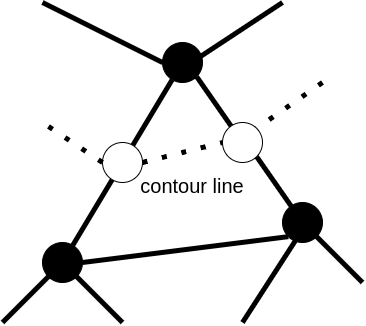
\includegraphics[width=0.5\textwidth]{contourline.png}
\caption{Create contour lines from intersections with triangles}
\label{fig:my_label}
\end{figure}




\section{Filled contour plotting algorithm}
FilledContourPlotPanel.java draws filled contour lines. The constructor obtains the triangle vertices and the scalar values from the vtk file and the color map object from the csv. The completed filled contour is scaled to fit the size of the JPanel and padding is added.
\subsection{Selecting vertices within a triangle}
Run a loop over the maximum and minimum x,y values of the triangle. Calculates whether a certain vertex p = (x, y) is included in a triangle using the cross product of vectors in isPointInTriangle() method. For each side of the triangle, compute the cross product of the side vector and the vector from point p to each vertex of the triangle. The sign of this cross product (positive, negative, zero) determines which side of each side the point p is on. Check the sign of each cross product, and if point p is on the same side of all sides (all positive or all negative), then the point is inside the triangle.
\subsection{Specify color for each vertex}
Once it determine that point p is located within the triangle, it determine the color of point p. Find the color of each vertex of the triangle, the point p, and the area ratio of the triangle formed by the two vertices. The color components (red, green, blue) of each vertex are weighted by area ratio and added. This determines the color of the given point p.
\begin{figure}[h]
\centering
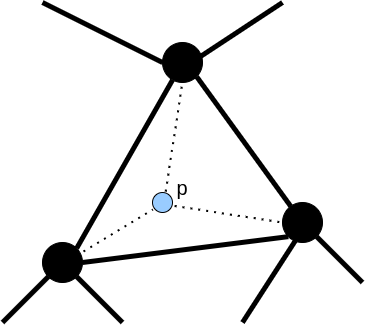
\includegraphics[width=0.5\textwidth]{filledcontourline.png}
\caption{Create filled contour lines}
\label{fig:my_label}
\end{figure}

\section{GUI}
The GUI is created with Swing. The JFrame contains a list for the user to specify the isoValue and a panel to display the contour lines and filled contour lines. When the user selects a vtk file from the file chooser, ContourPlotMain.update() is called. update() reads the vtk file and reloads the fields of the contour panel object. Then run the overridden paintComponent() again by repainting the contour panel. The refreshList() method updates the list when the user adds or removes isoValues. 
\begin{figure}[h]
\centering
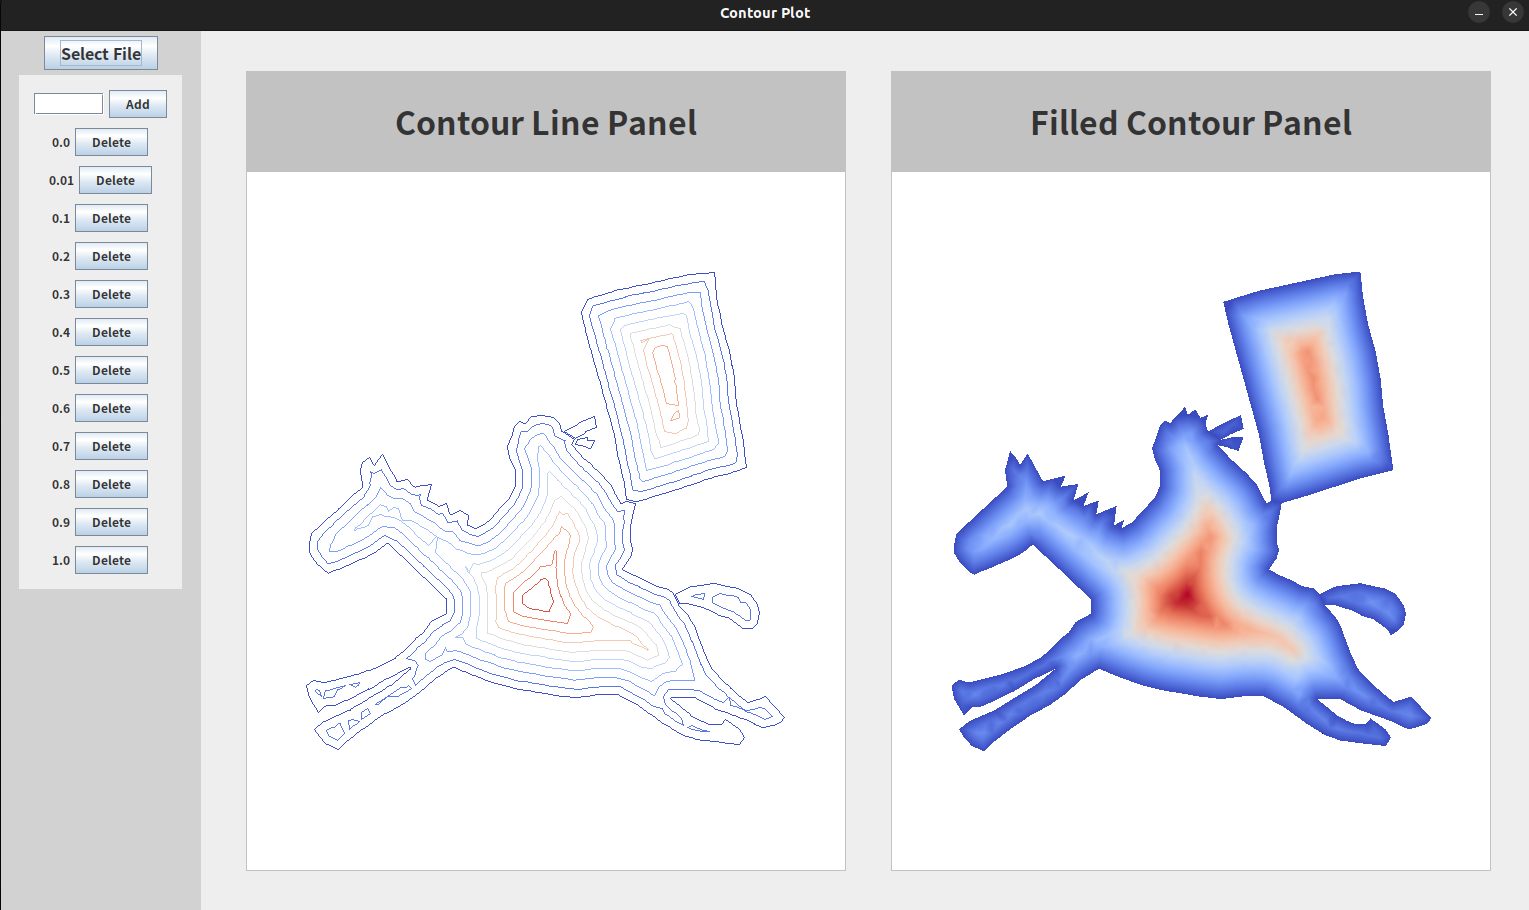
\includegraphics[width=1.0\textwidth]{gui.png}
\caption{Screenshot of GUI}
\label{fig:my_label}
\end{figure}

\begin{thebibliography}{99}
\bibitem{ref1}
\url{https://itandcfd.com/vtk_file_format/241/}
\bibitem{ref2}
\url{https://www.paraview.org/}
\bibitem{ref3}
\url{http://www.thothchildren.com/chapter/5b267a436298160664e80763}
\bibitem{ref4}
\url{https://www.javadrive.jp/tutorial/}
\bibitem{ref5}
\url{https://talavax.com/math-heron.html#gsc.tab=0}
\end{thebibliography}

\end{document}

